\documentclass[conference]{IEEEtran}
\IEEEoverridecommandlockouts
% The preceding line is only needed to identify funding in the first footnote. If that is unneeded, please comment it out.
\usepackage{cite}
\usepackage{amsmath,amssymb,amsfonts}
\usepackage{graphicx}
\usepackage{textcomp}
\def\BibTeX{{\rm B\kern-.05em{\sc i\kern-.025em b}\kern-.08em
    T\kern-.1667em\lower.7ex\hbox{E}\kern-.125emX}}
\begin{document}

\title{THE2\\
}

\author{\IEEEauthorblockN{Esref Ozturk}
\IEEEauthorblockA{\textit{CENG} \\
\textit{METU}\\
Ankara, Turkey \\
esrefozturk93@gmail.com}
}

\maketitle


\section{Introduction}
This report includes the discussions about CENG499 Machine Learning THE2 Homework \\

\section{Discussion}

\subsection{Feature Scaling Technique}

Min-Max scaling technique is used for scaling each  features to 0-1 range. Using min-max scaling, all different range features are scaled to the same range. Luckily there was no feature that has the same max and min so min-max scaling were used.

\subsection{Effects of the Different Architectures}

Following table shows accuracy scores for different iteration counts: \\

\begin{tabular}{l*{6}{c}r}
eta  & 1000 & 10000 & 100000 \\
\hline
3e-4 & 0.37 & 0.48 & 0.61 \\
1e-3 & 0.37 & 0.58 & 0.73 \\
1e-1 & 0.73 & 0.79 & 0.79 \\
\end{tabular} \\

As iteration count increases, the gap between learning rates are decreasing. Small learning rates are causing the accuracy to increase very slowly. If we want to use small learning rates, we should increase the iteration count.

\subsection{When to Stop Updates}

As it can be seen in the previous subsection, all lines are converging after some amount of epochs. We can stop updated there.


\subsection{Training and Validation Sets}

Using cross validation better learning rate can be selected. Also learning rate should be considered together with iteration count since for bigger iteration counts, smaller learning rates are enough.


\section{Plots}

\subsection{No Hidden Layers}

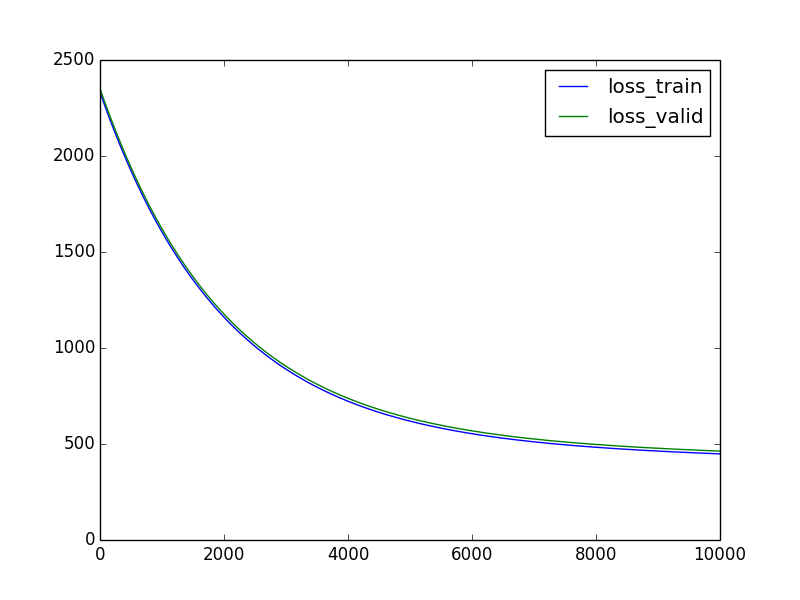
\includegraphics[width=0.5\textwidth]{set1-[].png}
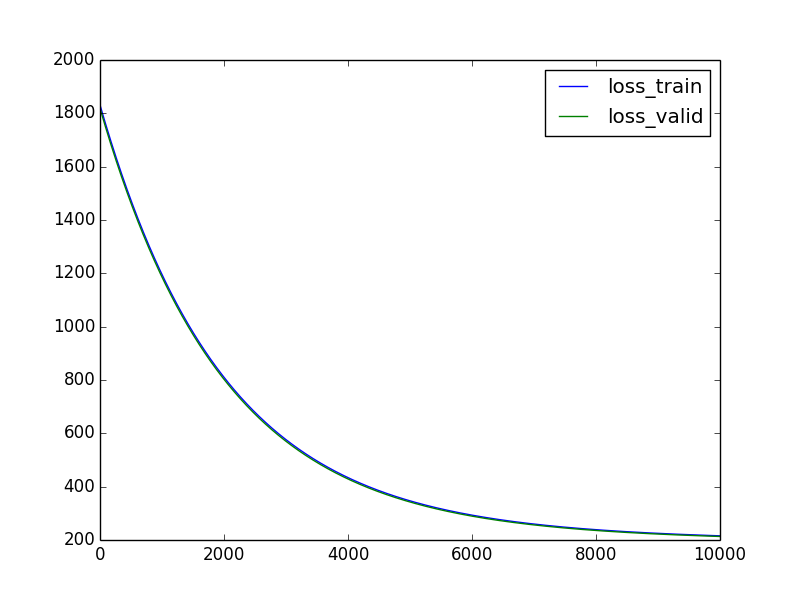
\includegraphics[width=0.5\textwidth]{set2-[].png}


\subsection{1 Hidden Layer with 1 Neuron}

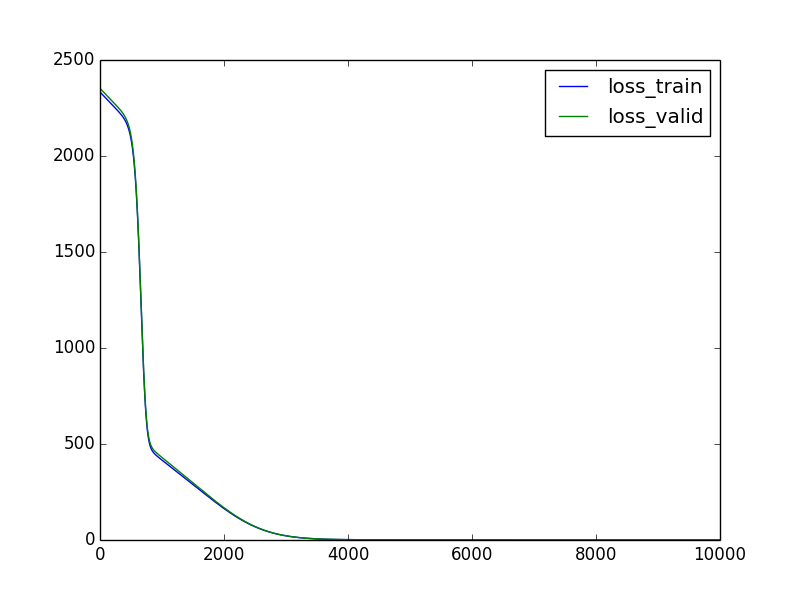
\includegraphics[width=0.5\textwidth]{set1-[1].png}
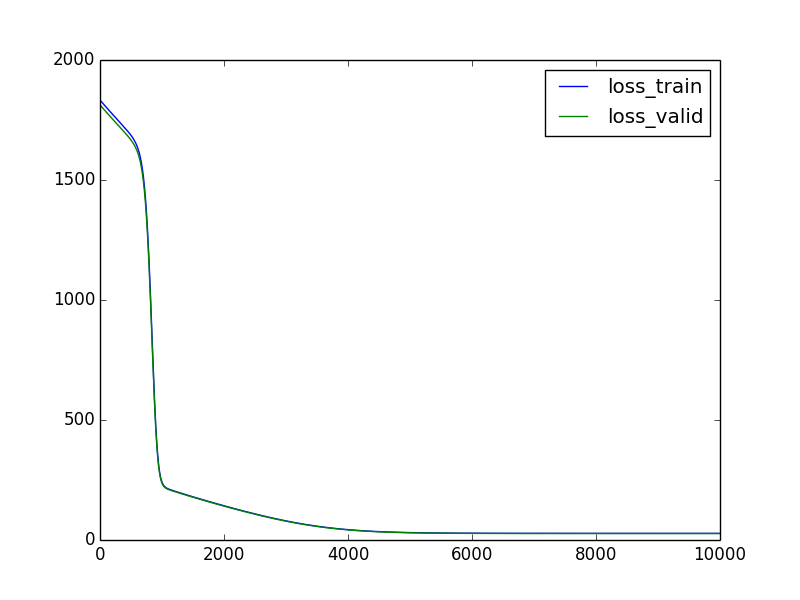
\includegraphics[width=0.5\textwidth]{set2-[1].png}


\subsection{1 Hidden Layer with 3 Neurons}

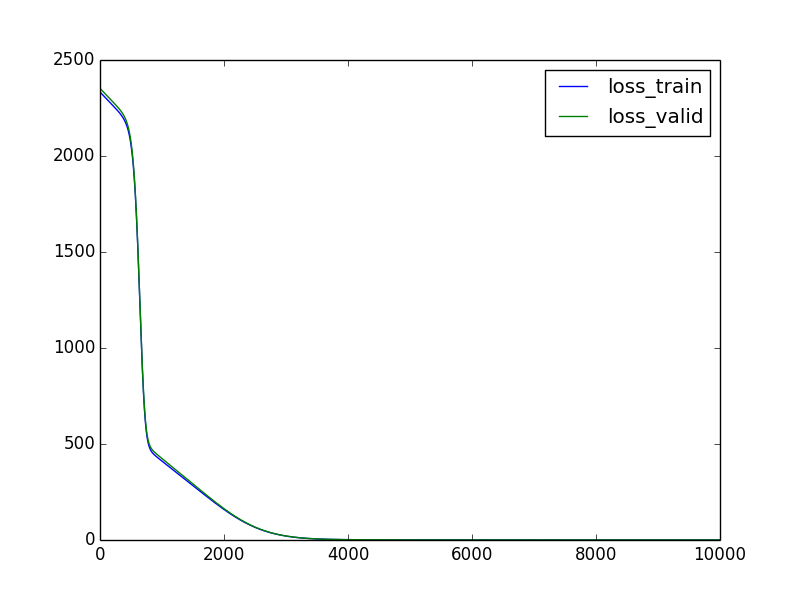
\includegraphics[width=0.5\textwidth]{set1-[3].png}
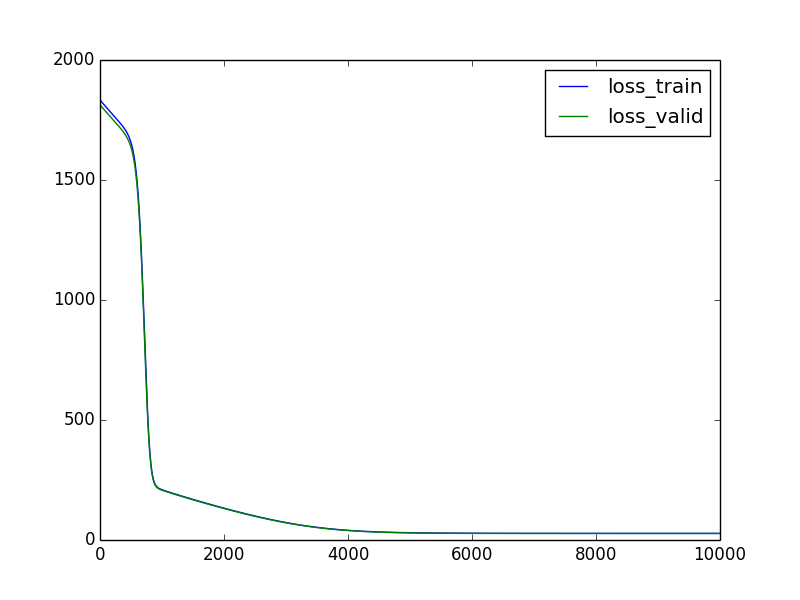
\includegraphics[width=0.5\textwidth]{set2-[3].png}

\subsection{2 Hidden Layer with 3 Neurons}

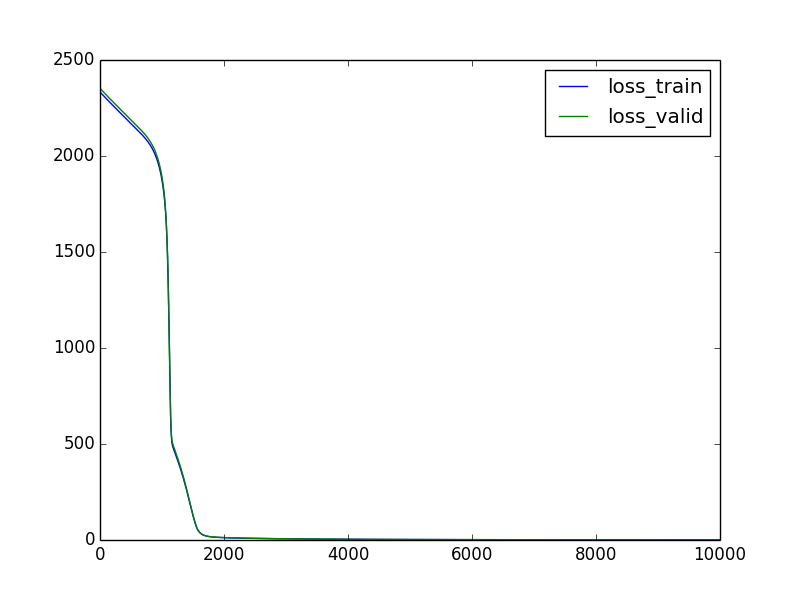
\includegraphics[width=0.5\textwidth]{set1-[3,3].png}
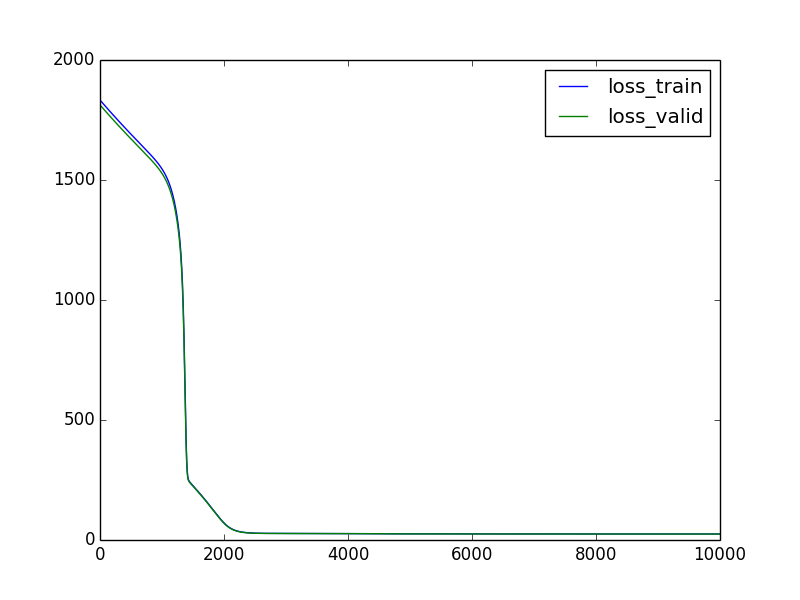
\includegraphics[width=0.5\textwidth]{set2-[3,3].png}

\subsection{3 Hidden Layer with 3 Neurons}

\includegraphics[width=0.5\textwidth]{set3-[3,3].png}
\includegraphics[width=0.5\textwidth]{set3-[3,3].png}



\section{Conclusion}
Since the dataset  was consisting of independent variables, logistic regression was very handy at analyzing it.

\end{document}
